\chapter{Read Error Correction}
\label{chap:read-error-correction}

Read data used as an input to many assembly algorithms contain plenty of errors, such as wrongly read bases. To make the data usable for assembly, an error correction step is required. However, it does not remove all the errors and assembly algorithms must cope with that fact, especially when dealing with read ends.

Currently, two different approaches are used to correct read errors, and both are based on transforming individual reads into series of k-mers. One is based on detecting errors as low covered edges (or paths) in a de Bruijn graph, the other works with a k-mer frequency distribution. During development of our algorithm presented in this thesis, we made several attempts to implement an error correction algorithm based on de Bruijn graphs. Since we use these graphs also during assembly performing error corrections on them seemed to be a natural choice. Although they definitely helped to improve the quality of input reads, all our attempts performed worse compared to the k-mer frequency distribution approach.

In the end, we decided to adopt the error correction algorithm used by the \texttt{fermi-lite} library \cite{fermi-lite} and based on k-mer frequency disbribution. This chapter describes both approaches.

\section{De Bruijn Graphs}
\label{sec:ec-de-bruin-graphs}

This method transforms the input set of reads into a de Bruijn graph in a way very similar to one used by our assembly algorithm. Although implementation details may differ, the basic idea is the same: each read mapped to certain active region is divided into a sequence of k-mers, each k-mer serves as a vertex and the edges follow the k-mer order within the sequence. Reference sequence, covering the active region, may also be included in the graph.

The basic assumption is that errors produce unique k-mers and thus also
nodes and edges with low coverage. Low-covered edges with source vertices that have output degree greater than one are especially interesting. A change of even a single base can divert a read path through edges with higher read coverage. The locality of the change depends on the k-mer size used.

A simple example demonstrating the main idea behind the method is displayed in Figure \ref{fig:error-correction-db}. Many reads share a sequence of \texttt{TTGCGCTAA}. However, there is also a single read that contains one error --- \texttt{TTGC{\textcolor{red}{A}}CTAA}. The de Bruijn graph shown on the figure uses k-mers 4 bases long. Combination of both sequences produces a standard bubble.

If the bubble was supported by reasonable amount of reads, it would be treated as a SNP. However, because there is only one supporting read, it may be reasonable to consider its divergence from other reads as an error, and to correct it, so the read path would follow more populated edges. When the correction is done, the resulting graph becomes linear, as shown on the right side in Figure \ref{fig:error-correction-db}.

\begin{figure}[h]
	\centering
	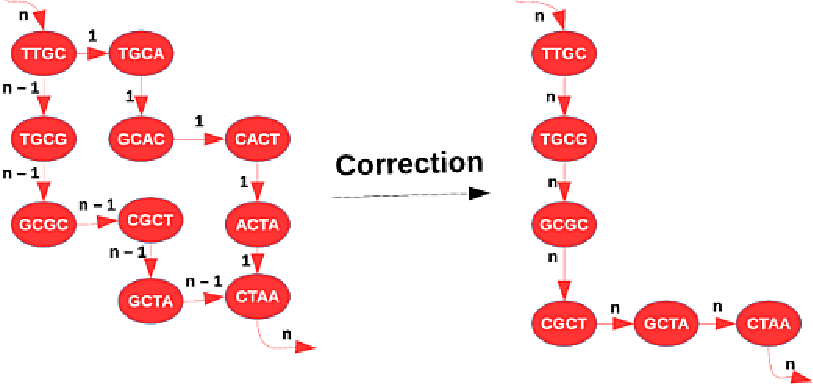
\includegraphics{img/error-correction-db.pdf}
	\caption{Simple examle of a read error detection by utilizing De Bruing graphs}
	\label{fig:error-correction-db}
\end{figure}

\section{K-mer Frequency Distribution}
\label{sec:ec-kmer-frequency-distribution}

The method is based on an assumption that k-mer frequency distribution of an error-free read set has certain properties. Especially, frequency of most of the k-mers is from 20 to 40, k-mers with other frequencies are very rare. Figure \ref{fig:kmer-frequency-distribution} shows the frequency distribution for an error-free read set and for a read set with error rate 1 \%. 

As can be deduced from the figure, errornous read sets have less k-mers with frequency between 20 and 40 and contain large amounts of unique or low-frequency ones. The idea behind the correction algorithms based on this method is to transform the low-frequency k-mers in order to move their frequency into the desired interval. Especially k-mers covering bases with low qualities are subjects to changes.

This approach is also used by the \texttt{fermi-lite} software and is covered in the next section.

\begin{figure}[h]
	\centering
	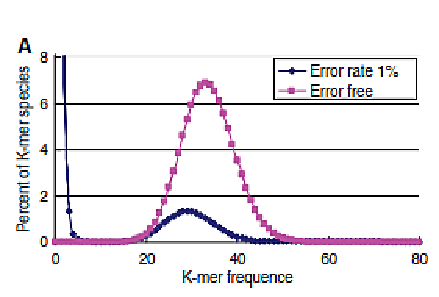
\includegraphics{img/kmer-frequency-distribution.pdf}
	\caption{K-mer frequency distribution for errornous and error-free read sets}
	\label{fig:kmer-frequency-distribution}
\end{figure}

\section{The Fermi-lite Approach}
\label{sec:fermi-lite}

\texttt{Fermi-lite} is a standalone C library as well as a command-line tool for assembling Illumina short reads in regions from 100 bp to 10 million bp in size. It is largely a light-weight in-memory version of \texttt{fermikit} without generating any intermediate files [from its GitHub]. Results of the assembly are not produced in the VCF format, but rather as a graph. Read error corrections are not the main goal of the project, although this step is definitely required for a successful assembly.

We have successfully extracted the error correction algorithm from the project. The implementation should work well on multiprocessor systems and trades performance over memory consumptuion. The algorithm proceeds in the following steps:
\begin{itemize}
\item \textbf{Preprocessing}. The input read sequences are divided into k-mers, k-mer frequencies are calculated.
\item \textbf{Error correction}. The problem is reduced into a shortest path graph problem and is solved by a kind of Dijkstra algorithm.
\item \textbf{Unique k-mer filtering}. Unique k-mers introduced during the error correction phase are removed from the read sequences.
\end{itemize}
 
\subsection{Data Preprocessing}
\label{subsec:fermi-data-preprocessing}

The main goal of the preprocessing phase is to compute frequencies for all k-mers found in the input read set. The frequencies are computed by inserting the k-mers into a k-mer table. During this phase, several terms related to k-mers and their occurrences are introduced:
\begin{itemize}
\item A k-mer occurrence is defined as \textit{high quality} one if quality of all bases covered by it is greater than certain threshold (set to 20 by default). If not all bases satisfy this condition, the occurrence is considered as \textit{low quality}.
\item A k-mer is considered \textit{solid} if its frequency is greater than certain threshold.
\item A k-mer is considered \textit{unique} if it its frequency is zero.
\item A k-mer is referred as \textit{absent} if it its frequency is is below certain threshold.
\end{itemize}
K-mers are implemented as four 64-bit integers,, with structure shown in Figure \ref{fig:fermi-kmer-structure}. Each base is represented by two bits. That gives limitation for maximum k-mer size to 64. The first 64-bit integer stores least signifficant bits of the k-mer bases, the second contains their most signifficant bits. The bases are stored in an opposite order --- the first base resides in bits k-1, the second to k-2 and so on. The second two integers store the same content, but with different order --- the first base is stored in bits 0, the second in bits 1 etc. Such a k-mer form is redundant; only two 64-bit integers are required to hold all the necessary information. The error correction algorithm actually uses the two-integer representation quite often.

Such a represetantion allows quick appends or individual base changes. To append a base into the first two integers, they just need to be shifted by one to the left, ORed with the new base, and ANDed with $2^k-1$ to set the unused bits to zero.

\begin{figure}[h]
	\centering
	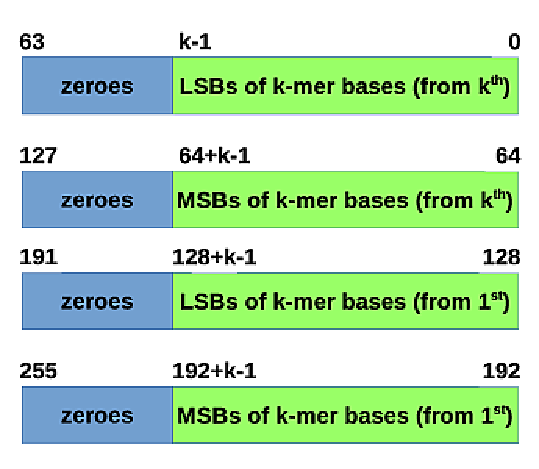
\includegraphics{img/fermi-kmer-structure.pdf}
	\caption{K-mer representation used by the \texttt{fermi-lite} project}
	\label{fig:fermi-kmer-structure}
\end{figure}

The k-mer table is actually a set of $2^{l_pre}$ khash tables. When a k-mer is being inserted or looked up, $l_pre$ bits of its data are used to select the table and the rest serves as an input to the hash function. $l_pre = 20$ by default. This representation of the k-mer table increases overall memory consumption, but has great impact on its performance in parallel environemnts. 

The table uses 14 bits to track occurrences of each k-mer. Lower 8 bits count low quality occurrences, higher 6 bits are used by high quality ones. The counting stops on values of 255 and 63, no integer overflow happens. The table actually stores their hashes and occurrences, rather than full k-mers. Hence, distinct k-mers may be treated as one, since the table may use up to $l_{pre}$ (20 by default) of k-mer content to choose the right khash table, and up to 50 bits may be stored as a key. That means, key colisions may be avoided if the k-mer size drops below 35 (the table actually has a different hash function for k-mers size below 33).

After the insertion stage, a k-mer frequency distribution is computed individually for low quality and high quality occurrences. The most common frequency is named \textit{mode} and is used during the second and third pahse of the algorithm.

All phases of the algorithm are partialy driven by its parameters. Table \ref{tab:fermi-parameters} provides a short description of them.

\begin{table}[h]
\begin{center}
\caption{Parameters of the \texttt{fermi-lite} algorithm}
\label{tab:fermi-parameters}
\begin{tabular}{| r | r | p{5cm} |}
\hline
Parameter & Default value & Description \\
\hline
$k$ & - & K-mer size. By default, this value is set to the base-two logarithm of the total number of bases. \\
\hline
$q$ & 20 & Base quality threshold used to recongize high quality content from low quality one. $P(error) = 10^{-\frac{q}{10}}$ \\
\hline
$min\_cov$ & 4 & Mimimum frequency for solid k-mers. \\
\hline
$win\_multi\_ec$ & 10 &  \\
\hline
$l_{pre}$ & 20 & Number of khash tables in the k-mer table, defined as $2^{l\_pre}$ \\
\hline
$min\_trim\_frac$ & 0.8 &  Defines how long the sequence of solid k-mers must be in order not to remove the read during unique k-mer filtering. \\
\hline
$w_{ec}$ & 1 & Participates in the weighing function used in the error correction step.\\
\hline
$w_{ec\_high}$ & 7 & Participates in the weighing function used in the error correction step. \\
\hline
$w_{absent}$ & 3 & Participates in the weighing function used in the error correction step. \\
\hline
$w_{absent\_high}$ & 1 & Participates in the weighing function used in the error correction step. \\ 
\hline
$max\_path\_diff$ & 15 & Participates in the weighing function used in the error correction step. \\ 
\hline
\end{tabular}
\end{center}
\end{table}

\subsection{Error Correction}
\label{subsec:fermi-error-correction}

The error correction is performed separately for each read sequence. The correction problem is transformed into a shortest-path search in a layered oriented graph. Vertices represent individual k-mers, edges connect adjacent ones and their weights reflect the cost of transforming one k-mer to another. The weight function is defined by formula
\begin{gather}
	w(k_i) = w_{absent\_high}*nhq(k_i) + w_{absent}*nlq(k_i) + w_{ec}*ec(k_i) + w_{ec\_high}*bq(k_i) \\
	nhq(k_i) = 0 iff k_i is a high-quality k-mer, 1, otherwise \\
	nlq(k_i) = 0 iff k_i is a low-quality k-mer, 0 otherwise \\
	ec(k_i) = 0 iff k_i introduces no error correction, 1 otherwise \\
	bq(k_i) = 0 iff the last base of k_i has quality above q, 1 otherwise
\end{gather}

The search algorithm used is a Dijksra one and its main loop can be decomposed into the following steps:
\begin{itemize}
\item Retrieve the vertex with lowest price, and its k-mer from the heap.
\item by separately appending \texttt{A}, \texttt{C}, \texttt{G}, and \texttt{T} to the k-mer, touch the adjacent vertices on the next layer and compute the cost of their connections.
\item Insert the newly created vertices into the heap.
\end{itemize}

Each path from the starting vertex to a vertex in the last layer represents one possible corrected part of the read sequence. Four such paths are computed. The path computation stops if a gap greater than $max\_path\_diff$ is detected in their costs.

\subsection{Unique k-mer Filtering}
\label{subsec:fermi-unique-kmer-filtering}

The error correction phase may produce unique k-mers which, as Figure \ref{fig:kmer-frequency-distribution} indicates, are not desirable. The \texttt{fermi-lite} library attempts to get rid of such k-mers. Each corrected read sequence is processed separately (and in parallel with others). 

At first, the longest k-mer sequence covered by non-unique k-mers is found. Denote its length, in k-mers, as $n$ and the read sequence length as $l$. Then, the read sequence between the read start and the first base covered by the found k-mer sequence is removed from the read. If the read is covered only by non-unique k-mers, nothing is removed, since the k-mer sequence covers the whole read. Howerver, if the following is true:
$$
\frac{n + k - 1}{l} < min\_trim\_frac
$$
the read is removed from the read set. This case includes also zero-length k-mer sequences that appear when the read contains unique k-mers only.